\documentclass{article}
\usepackage[UTF8]{ctex}
\usepackage{geometry}
\usepackage{multirow}
\usepackage{natbib}
\geometry{left=3.18cm,right=3.18cm,top=2.54cm,bottom=2.54cm}
\usepackage{graphicx}
\pagestyle{plain}	
\usepackage{setspace}
\usepackage{enumerate}
\usepackage{caption2}
\usepackage{datetime} %日期
\renewcommand{\today}{\number\year 年 \number\month 月 \number\day 日}
\renewcommand{\captionlabelfont}{\small}
\renewcommand{\captionfont}{\small}
\begin{document}

\begin{figure}
    \centering
    
\includegraphics[width=8cm]{upc.png}

    \label{figupc}
\end{figure}

	\begin{center}
		\quad \\
		\quad \\
		\heiti \fontsize{45}{17} \quad \quad \quad 
		\vskip 1.5cm
		\heiti \zihao{2} 《计算科学导论》个人职业规划
	\end{center}
	\vskip 2.0cm
		
	\begin{quotation}
% 	\begin{center}
		\doublespacing
		
        \zihao{4}\par\setlength\parindent{7em}
		\quad 

		学生姓名:\underline{\qquad  何为 \qquad \qquad}

		学\hspace{0.61cm} 号:\underline{\qquad 2007020213\qquad}
		
		专业班级:\underline{\qquad 本研(AI)2001班 \qquad  }
		
        学\hspace{0.61cm} 院:\underline{计算机科学与技术学院}
% 	\end{center}
		\vskip 1.5cm
		\centering
		\begin{table}[h]
            \centering 
            \zihao{4}
            \begin{tabular}{|c|c|c|c|c|c|c|c|c|}
            % 这里的rl 与表格对应可以看到,姓名是r,右对齐的;学号是l,左对齐的;若想居中,使用c关键字。
                \hline
                \multicolumn{5}{|c|}{分项评价} &\multicolumn{2}{c|}{整体评价}  & 总    分 & 评 阅 教 师\\
                \hline
                自我 & 环境 & 职业 & 实施 & 评估与 & 完整性 & 可行性 &\multirow{2}*{} &\multirow{2}*{}\\
                分析& 分析& 定位 & 方案 & 调整 & 20\% & 20\% & ~&~ \\\            
                10\% & 10\% & 15\% & 15\% & 10\% & &  &~ &~\\
                \cline{1-7} 
                & & & & & & & ~&~ \\
                & & & & & & & ~&~ \\
                \hline      
            \end{tabular}
        \end{table}
		\vskip 2cm
		\today
	\end{quotation}

\thispagestyle{empty}
\newpage
\setcounter{page}{1}
% 在这之前是封面,在这之后是正文
\section{自我分析}
	%自我分析即对自己进行全方位、多角度的分析,目的是认识自己、了解自己。只有认识了自己,才能对自己的职业做出正确的选择,才能选定适合自己发展的职业生涯路线,才能对自己的职业生涯目标做出最佳抉择。\par
	%自我分析包括:\par
\subsection{自然条件}


\begin{table}[h]
	\centering
	\caption{个人自然条件分析}
	\begin{tabular}{cl}
		% 这里的rl 与表格对应可以看到,姓名是r,右对齐的;学号是l,左对齐的;若想居中,使用c关键字。
		\hline
		方面 & 个人信息 \\
		\hline
		性别 & 男 \\ 
		年龄 & 19岁 \\
		身体条件 & 身高一米七左右,体重60kg左右,BMI指数优秀,眼睛近视,\\
		        &  身体留有几处伤疤,但不影响正常生活\\
		健康状况 & 身体健康状况良好,不吃烟,很少喝酒,偶尔熬夜外没有其他恶习\\
		居住城市 & 居住在四线城市,毕业以后工作方面暂时没考虑留在家乡发展\\
		\hline
	\end{tabular}
	\label{table1}
\end{table}


%性别、年龄、身体条件、健康状况、居住城市等。\par
%男;19岁;身高一米七左右,体重58kg左右,BMI指数优秀;身体健康状况良好,不吃烟,很少喝酒,偶尔熬夜外没有其他恶习;居住在四线城市,毕业以后工作方面暂时没考虑留在家乡发展;眼睛近视,身体留有几处伤疤,但不影响正常生活。
\subsection{性格分析}
\textbf{\textit{优势:}}\par 
性格外向,善于沟通,便于获得更多的资源;\par
工作注意细节,追求完美,目标够高;\par
好胜,喜欢接受挑战,不愿轻易放弃;理性,能够冷静下来思考;\par
抗压能力强,困难的时候,有自己的方式释放压力,克服困难;\par
自立,能够驾驭大学生活学习,凡是自己能解决掉的问题,不愿意轻易劳烦别人;\par
生活学习态度多为谦和,脾气好,不愿意与人争吵,听得进别人劝告;\par
三观正,有一定的辨别力,偏好那些实实在在的朋友;\par
喜欢与别人交流,尤其是与优秀的人,想学到更多的东西,但是有时候也喜欢一个人待着,一个人思考。\par
 
\textbf{\textit{劣势:}}\par
持久力不行,易浮躁;\par
大局观的把控不是很好;\par
在一些方面显得很犟;\par
视觉不够敏感,不如听觉;\par 
不善于与记忆,背诵;\par
性子直,有时候说话不过脑子;\par
脾气太好,有时候不能当机立断;\par
有些时候偏强势,尽管有刻意控制,但平时在与别人相处中偶尔还是会不经意给人压抑。\par

\textbf{内方外圆是我的目标}\par
\textbf{(优势和劣势之分只是我个人就目前阶段所需分析得出,但个人觉着,并不意味着好坏之分)}

\subsection{教育与学习经历}
小学期间爱玩,有较好的学习资源没有利用好,那个时候太小,与努力鲜花掌声比起来,觉着倒数趴在那更舒服一些;到了初中的时候所处班级的教育资源就不是那么好了,在一群不是很优秀的同龄人之中能够凭借自己的小聪明取得一点成绩,那个时候为了保持自己优越感,也用心学过一段时间,有了一定的数学英语基础;上了高中,教育资源一般,但身边较初中有一部分大佬,还是为了保持自己的优越感,在努力学习,但是那个时候还是因为性格缺陷,持久力不行,那时候的状态就是想起来了就拼一段时间,有点成绩了就会飘一段时间,导致成绩也不是很稳定,性格里也埋下了浮躁的种子,但那个时候要强;学习上和性格上正真有所成长和升华的是高四的时候,复习的那一年凭借着上一年还算不错的成绩分到了县级重点班中的重点班,真正见识到了一些牛人,那一年,在那个班,成绩上没有一点可以骄傲的地方,让我真正看到了自己的不足,压力也从四面八方迎面而来,内心备受煎熬,在折磨中磨炼了棱角,我个人觉着是我自己人生的一种沉淀,是我强与别人的地方。\par
相比较大学中其他的同学,我没有参加过其他的学习培训,到现在只是按部就班的学着应该学习的东西,所见的世面太小,大学期间真的迫切需要扩充自己的知识。\par
在这里尤其需要强调的是在多年的教育生涯中,语文一直处于一个不是很重要的地位,我在此方面精力的倾注也是应其当时的价值,不多,从一开始就留下了隐患,也一直没去弥补,导致现在个人对文字的敏感度和记忆力较普通人差了很多,而且一些基础知识,即所谓的常识,远远不够,这点是我的短板,需要弥补,而我能想到的是通过读书去弥补。\par
\subsection{工作与社会阅历}
小学担任课代表,初中兼任多课课代表,我工作足够认真,自我感觉很讨老师喜欢,高中担任三年班副,班级饭卡充值这活我干了三年,没出现一次事故(自认为和钱打交道的活都不好干),高中班级的晚会,活动大多都是组织者和谋划者,在组织与策划能力上,自认为高出同龄人;社会实践的话很少,能想起来的是以前应学校要求做过采访;上初中的时候就开始想出去打暑假工赚钱,那个时候年级小,个子也不高,没人要,但是在父母的工作单位上待了一个月,打打杂工,那个时候父母是想用工资吸引,不让我整体在家玩游戏,最终确确实实,从那里出来后感受到赚钱不容易,体会到父母的艰辛,没提过要钱的事。目前截止,我这种锻炼有过三次,第一次是初一,初三暑假去了一个月,高二暑假去了半个月,这三次锻炼,是正真意义上的成长,如果说第一次是被引导,后两次绝对是自愿,目的就是为了锻炼,结果也确实有锻炼的作用。\par
\subsection{知识、技能与经验}
善于与人沟通交流;\par 
在管理方面有一定的经验;\par 
恋爱方面有一定的经验; \par
会基础的Word/Excel表格操作;\par 
有一定的识人能力,一定的判断力;\par 
学习能力处于我现在所处环境的平均水平之上。\par 
(仔细分析一下,在知识,技能方面和别人有一定的差距,优势的话可能突出在能力和经验方面,而大学,迫切需要把能力和经验沉淀为知识和技能)\par 

\subsection{兴趣爱好与特长}
运动:慢跑,羽毛球;\par
学习:编程,PR,PS,Word/Excel;\par 
游戏:LOL。\par 
\par
\section{环境分析}
%环境分析主要是评估周边各种环境因素对自己职业生涯发展的影响。每一个人都处在一定的环境之中,职业发展必然要受到所处环境的影响,只有充分了解和把握所处环境的现状、特点、发展变化趋势,才能做到在复杂的环境中避害趋利,使你的职业生涯规划具有实际意义。\par
%环境分析包括:\par
\subsection{社会环境分析}
%政治形势、经济形势、就业形势等。\par
本专业人工智能类,目前国家重视,市场需求高,就业前景好。政策近几年一直在优化,未来可期。\par 
但是在社会上本专业人员供大于求,遍地都是程序员,而国家,企业,市场需要的是尖端人才,要想出人头地,有所成就,就得成为专业人才,而不是专业人员;人才的很重要的标准是创新能力,创新的话先得具备必要的基础技能,然后得多做实验,从实践中反思,发现不足,设法提升;大学是个很好的平台去学习,去时间,去试错,去培养创新能力。\par 
大学地理位置:青岛市我所了解到的是现在很少IT高企,毕业后我应该会考虑去外面发展。\par
\subsection{家庭环境分析}
%婚姻状况、经济状况、家人期望、家族传统等。\par

感情方面:家人潜移默化的传递给了我正确的爱情观,在情感方面对我也没做要求,我个人对待感情则是被动等待,全力出击,近几年应该不会做太高要求;还有从我之前的感情经历来看,我在自己的感情方面可能不是驾驭的很好,一旦陷入进去很爱钻牛角尖,对个人的生活学习影响很大,我需要时间去沉淀自己。\par
 \par
经济状况:毕业后甚至毕业前几年就要实现经济独立,所有经济方面的问题,自己一定要想办法自己独立解决;之前几年在工地上锻炼过,深知赚钱不易,而且父母现在念过半百,尽早的实现经济独立也算大学的一个目标。\par
 \par
 
家人期望:家人要求不太高,正常情况,不会左右我个人的决定,未来的发展去向,全权掌握在我自己的手上;父母家人多是指点与建议。\par
 \par
家族传统:家庭历代务农,我这代是转折点,我未来的何去何从,全部掌握在我自己手上,家人多是指点为人处世方面,其他方面干涉的少,哥哥是从事本专业行业,能够给到我这方面的指点,但哥哥对我也多是指点,很少干涉。\par
 \par
家庭地理位置:家庭位处四线城市,而且河南省没看到有哪些城市有本专业大展宏图的机会,目前来看毕业后应该不会回家乡发展,想去的应该是上海,深圳等一线城市,上海离家近而且我很看好这个城市,深圳是因为那边有亲人,而且那边大多用得上本专业的公司,至于北京,一是离家太远,二是环境条件不是特别好,因此不是很想去北京发展。\par
 \par
\subsection{职业环境分析}
%行业现状及发展趋势;职业的工作内容、工作要求、发展前景等。\par
行业现状和发展趋势:人工智能类,个人觉着现在目前的技术还不是很成熟,在很多方面还得实验优化,但是发展趋势发展前景很好,预估等我们毕业的时候,人工智能大体上一个有模有样了;\par
\textbf{(配当前某IT公司对招聘人员要求)}\par
工作内容:算法,软件开发;\par
工作要求:学历,掌握精通各种编程语言,交涉能力,社交能力;\par 

a. 本科及以上学历,硕士博士以及985/211大学优先。计算机科学、数学、控制论、博弈论、运筹学、统计学等相关专业,有扎实的数理分析基础并有交叉领域研究经验的优先;\par
b. 强烈的技术热情和学习渴望,对技术驱动业务有不懈的追求,希望能够树立行业影响力;\par
c. 独立思考、追求创新,有良好的技术洞察力、商业敏感度和优秀的数据分析技能,积极主动,有较强的团队合作精神;\par
d. 熟悉常用数据挖掘和机器学习算法(Online Learning, Deep Learning, Multi-task learning, MultiModal Machine Learning, Reinforcement learning),图像/视频内容理解技术,个性化搜索推荐技术,图算法等;
e. 熟练使用Python/Java/C++/Shell/SQL等编程语言;\par
f. 有TensorFlow/Caffe/Keras/Theano等深度学习框架实践经验,有大数据应用经验者优先;\par
g. 对人工智能相关领域有大量研究或实践经验,有实际成果并发表在国际顶级会议、期刊者优先;\par
h. 良好英文沟通能力者优先。\par
社会需求决定学习方向。
\subsection{地域与人际环境分析}
工作城市的气候水土、文化特点、发展前景;人脉与人际关系等。\par

未来工作城市考虑:\par
1,上海:上海这个城市我非常看好,在该地本专业未来会有很大的发展前景\par 
\begin{figure}[h!]
\centering
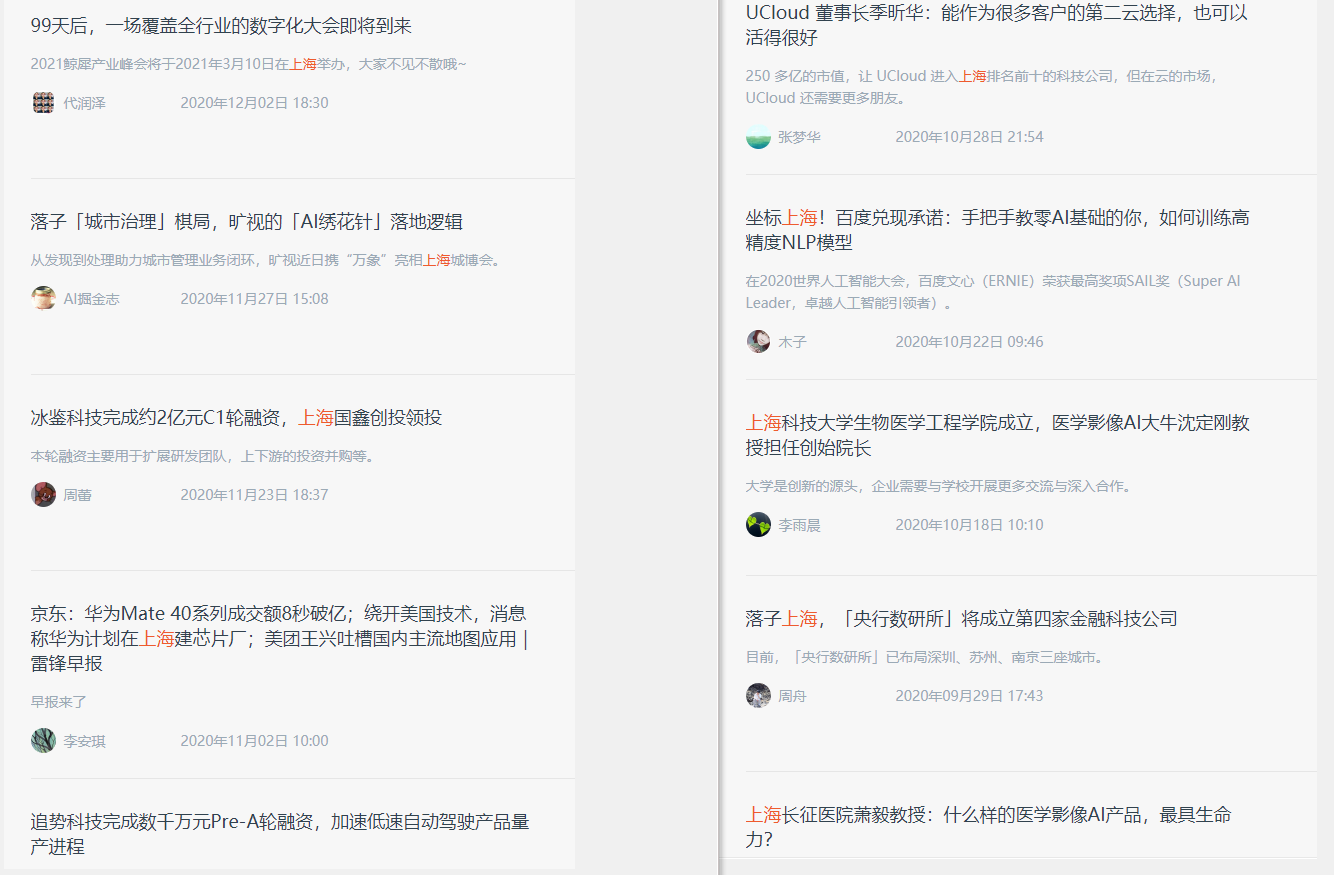
\includegraphics[width=10cm, height=5cm]{1}
\caption{上海}
\label{fig:1}
\end{figure}
另外是因为上海离家很近,而且上海的环境比较适宜居住。

2,深圳:主要是因为自己兄长在深圳发展,刚刚毕业的几年可能需要兄长带着,而且深圳我也去了几趟,觉着由于地方政府对环境的监管非常的严格,深圳的环境很不错,除了潮湿一点意外,还是蛮适合居住的。\par
(其他城市还在考虑,而且现在城市的考虑只是粗略化,因为等我毕业,可能又是另一番趋势,但是北京的话,目前不考虑,一是离家太远,二是环境不太好,而且青岛本地的话,目前也没有考虑,主要是青岛没有太多的IT大公司)

\section{职业定位}
%在准确地对自己和环境做出了分析之后,确定适合自己行业和有实现可能的职业发展目标。职业定位时要注意与自己的自然条件、知识背景、技能特长、性格特点、兴趣爱好是否匹配,考虑与自己所处的环境是否相适应。职业定位决定了职业发展中的行为和结果,是制定职业生涯规划的关键,应当科学合理,具有可行性。\par
%职业定位包括:\par

\subsection{行业领域定位与理由}
大三计划选择的方向人工智能和大数据,行业领域也是这个方向;\par
理由:\par
1,人工智能和大数据的未来前景,等我们毕业的时候,预估又是一次浪潮,当然得做时代的弄潮儿;\par
2,家里的兄长已经从事软件开发领域,我想是一家人不能都学一样的,多一项技艺,多一种可能;\par
3,个人对人工智能的兴趣在学习的过程中,也是只增不减,我对它很信任,而且我也对自己的能力很信任。\par

\subsection{职业岗位起点定位与理由}
职业岗位起点定位:\par
从员工做起,毕业后的前几年一定是锻炼,将自己从大学学到的知识应用到工作的实战之中,这个年限预估一到三年,而且非常有必要,这也算是提前有个心理准备吧;\par
工资:年薪20-30万左右较为合理;考虑到本学校的平均年薪和最高年薪,再结合本人目前的专业知识能力,和市场上行情,综合定下的小目标;\par



\subsection{职业目标与可行性分析}
\par
%成果目标、经济目标、能力目标、职务目标等。\par 
\begin{enumerate}[(1)]
	\item 短期目标:(大学期间目标)\par
	适应大学生活,提升利用大学资源的能力;\par
	完成学业要求,熟练掌握专业知识,灵活运用专业技能,培养创新思维与能力;\par
	大学期间参加至少三项竞赛,其中省以上至少一项,至少一次出国留学;\par
	读书,磨炼自己的性格,养成好的习惯;\par
	构建自己的知识体系;\par
	规划未来职业走向;\par
	
	
	\item 中长期目标:(毕业后一到五年)\par
	大学与社会的灵活转化;(生活,专业知识,能力)\par
	稳定工作,年薪20-50万;\par
	稳定自己的情感与家庭;\par
	构建自己的知识体系;\par
\end{enumerate}
可行性分析:\par
综合当前本专业对学生要求与学校所能够提供的资源与社会的发展趋势,加上对自身的能力分析以及对身边人毕业几年发展的现实例子,对个人未来十余年的职业做出如此合理规划;\par
结合本学期所学所知,以及老师的启发,我另对个人的综合发展有了一定的规划。\par


\section{实施方案}
%在明确了职业定位后,要制定实现职业生涯目标的行动方案,不付诸行动,职业目标只能是一种梦想。实施方案是实现职业目标的保证,尽量考虑周全、具有可操作性。\par

%实施方案可以从以下角度考虑:\par
\begin{enumerate}[1、]
	\item 如何利用现有条件和自身优势以实现职业生涯目标。\par
	身体是革命的本钱,继续坚持锻炼,保持一个健康有活力的身体条件;\par
	充分利用自己寻找资源的能力,在大学里充分利用导员,老师,图书馆,以及周围同学家人等的这些资源;\par
	利用自己的学习能力,在这最好的年龄,学习能力最强的时候,一定要储备尽量多的知识技能;\par
	利用个人性格优势,多去尝试不同的挑战,快速成长。\par
	
	\item 如何克服缺点、弥补不足、增长知识、提高能力以实现职业生涯目标。\par
	多读书,提升对文中的铭感度,巩固自己的常识技能;\par
	多读书,让自己沉稳下来,对自己不足有清晰认识;\par
	多读书,多思考,构建自己的知识体系。 \par
	
	
	\item 如何处理人际关系和发展人脉以实现职业生涯目标。\par
	保持热情,多和人沟通,多交流,与人相处多谦让多体谅,利用好班长的职位,锻炼识人能力,结交更多的人;\par
	与人交流的过程中,我觉着谁也不是傻子,只要够实在,够认真,同学老师们都能感受的到,都愿意和你相处,而对你来说,正是这些人脉是大学最宝贵的财富,也是人生的一大笔财富。\par
	
	\item 如何处理工作与家庭、生活的关系以实现职业生涯目标。\par
	家和万事兴,家庭能够和睦,健健康康的,对自己的发展也有很大的帮助;\par
	趁着都还年轻,和家人多沟通,与家人多关心,有空和家人一起出去旅旅游,即是家人心灵的栖息也有利于未来发展。\par
	
	\item 如何处理释放工作压力、保证身心健康以实现职业生涯目标。\par
	利用兴趣:\par
	慢跑,散步;和朋友打打球;和朋友开开黑,打打游戏;一个人去图书馆读读喜欢的书等等\par
	这些对我个人排解压力都有很大的帮助。
	
\end{enumerate}
\par 

\section{评估与调整}
%由于影响职业生涯规划的因素很多,且大都处于动态变化之中,因此职业生涯规划应定期评估,并根据影响因素的变化和实施结果的情况及时作出调整,这样才能保证其行之有效。\par 
\subsection{评估时间}
每学年一次。\par
\subsection{评估内容}
可以从成果目标、经济目标、能力目标、职务目标等方面总结,确定哪些目标已按预期实现,哪些目标商未达到,对已实现的成果总结经验,对未完成的目标分析原因。\par
结合社会趋势,专业前景,以及已完成情况,对本职业规划进行合理的修改。\par
\subsection{调整原则}
应考虑与自身情况的匹配性、与环境的适应性、操作实施的可行性等。\par

\end{document}
